Las neuronas se comunican entre sí mediante la \textit{sinápsis} (ver el sitio web \cite{khanacademywebsite}). La \textit{sinápsis} es el punto de comunicación entre dos neuronas, o entre una neurona y una glándula. En la sinápsis, el disparo de un \textit{potencial de acción} en una neurona (la neurona \textbf{presináptica} o emisora), provoca la transmisión de una señal a otra neurona (la neurona \textbf{postsináptica} o receptora), lo que aumenta o disminuye la probabilidad de que la neurona postsináptica dispare su propio \textit{potencial de acción} (ver figura~\ref{fig:Sinapsis}). 
\begin{figure}[htbp!]
    \centering
    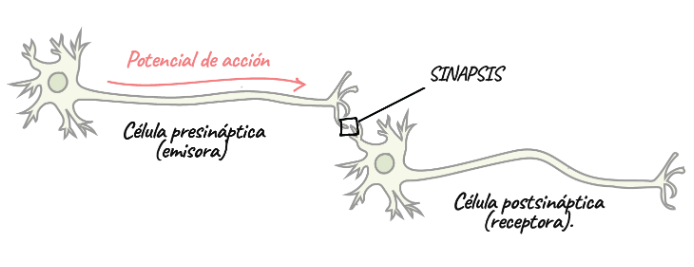
\includegraphics[width=10.0cm]{figures/Sinapsis.png}
    \caption{Sinápsis. Comunicación entre neuronas}
    \label{fig:Sinapsis}
\end{figure}
\section{Potencial de membrana}\label{section:Potencial_Membrana}
Las neuronas tienen, además del potencial de acción, un \textit{potencial de reposo} (potencial de membrana en reposo) (ver  el sitio web \cite{khanacademywebsite}). Si uno pudiera tomar las puntas de un voltímetro y colocarlas una en el exterior y otra en el interior de la membrana plasmática de una célula viva, se mediría una diferencia de potencial o voltaje al que se denomina \textbf{potencial de membrana}. El punto de referencia es el exterior de la célula. En la mayoría de las neuronas en reposo, la diferencia de potencial de la membrana es de 30 mV a 90 mV, con el interior de la célula más negativo que el exterior. Es decir, las neuronas tienen un \textbf{potencial de membrana en reposo} de -30 mV a -90 mV.
\begin{figure}[htbp!]
    \centering
    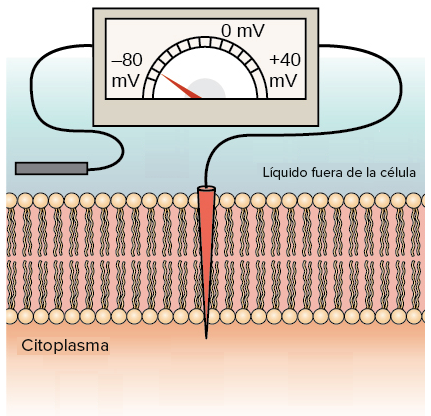
\includegraphics[width=4.5cm]{figures/potencial_membrana.png}
    \caption{Potencial de membrana}
    \label{fig:Potencial_membrana}
\end{figure}
El potencial de reposo de membrana está determinado por la distribución desigual de \textbf{iones} entre el interior y el exterior de la célula, y por las diferencias en la permeabilidad de la membrana hacia diferentes tipos de iones. En las neuronas y sus líquido circundante, los iones más abundantes son:
\begin{itemize}
    \item Cationes (iones con carga positiva): Sodio ($Na^+$) y potasio ($K^+$)
    \item Aniones (iones con carga negativa): Cloruro ($Cl^-$) y aniones orgánicos (proteínas y aminoácidos)
\end{itemize}
\newpage
En la mayoría de las neuronas, el $k^+$ y los aniones orgánicos se encuentran en concentraciones más altas dentro que fuera de la célula. En cambio, el $Na^+$ y el $Cl^-$ generalmente se encuentran en concentraciones más altas fuera de la célula (fig.~\ref{fig:concentracion_iones}). Esto significa que a través de la membrana existe un gradiente de concentración por la acumulación de partículas en mayor cantidad en un lado que en otro. Las partículas se difunden a favor del gradiente de concentración desde áreas de mayor concentración hacia áreas de menor concentración, hasta que estén igualmente distribuidas.
\begin{figure*}[h!]
        \centering
        \begin{subfigure}[b]{0.35\textwidth}
            \centering
            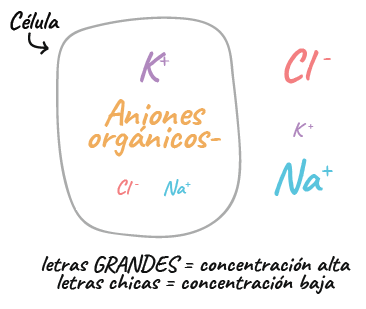
\includegraphics[width=\textwidth]{figures/concentracion_iones.png}
            \caption{Concentración de iones dentro y fuera de la célula}
            \label{fig:concentracion_iones}
        \end{subfigure}
        \hspace{1.5cm}
        \begin{subfigure}[b]{0.4\textwidth}  
            \centering 
            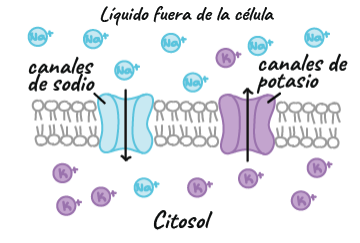
\includegraphics[width=\textwidth]{figures/canales_iones.png}
            \caption{Canales a través de los cuales los iones cruzan la membrana}
            \label{fig:canales_iones}
        \end{subfigure}
        \quad
        \caption{Concentración de iones y movimiento dentro y fuera de la célula}
\end{figure*}
Debido a su carga, los iones no pueden pasar directamente a través de las regiones de lípidos hidrofóbicos ("temerosos del agua") de la membrana, sino que lo tienen que hacer a través de \textit{canales de proteínas} especializados que proporcionan un túnel hidrofílico ("amigo del agua") que cruzan la membrana. Existen canales, llamados \textit{canales de filtración}, que están abiertos en membranas en reposo y canales que se cierran en neuronas en reposo y sólo se abren en respuesta a una señal.\\
Los canales iónicos que permiten solamente el paso de $k^+$ se llaman \textbf{canales de potasio} y los que permiten principalmente el paso del $Na^+$ se denominan \textbf{canales de sodio} (fig.~\ref{fig:canales_iones}).\\
El movimiento de iones $k^+$ a través de la membrana es el principal responsable del potencial de membrana de una neurona en reposo. Cuando hay una mayor concentración de $k^+$ dentro de la célula que en el líquido circundante y se abren los canales de potasio en la membrana, el $k^+$ comenzará a fluir por su gradiente de concentración hacia el exterior de la célula. Cada vez que un ión $k^+$ sale de la célula, el interior de la célula pierda una carga positiva. En el exterior de la membrana celular se acumula un ligero exceso de carga positiva y en el interior se acumula un ligero exceso de carga negativa. El interior de la célula se vuelve negativo a comparación del exterior y se establece una diferencia de potencial eléctrico en la membrana.\\
Cuando se establece la diferencia de potencial eléctrico en la membrana se dificulta que los iones $k+$ restantes puedan salir de la célula debido a que los iones $k^+$ de carga positiva son atraídos por los iones de carga negativa del interior de la célula y a su vez son repelidos por las cargas positivas del exterior. Todo esto se opone al movimiento en dirección del gradiente de concentración.\\
La diferencia de potencial en la membrana se acumula hasta que la \textit{fuerza eléctrica} que impulsa al $k^+$ de regreso a la célula sea igual a la \textit{fuerza química} que impulsa la salida del $k^+$ a través de los canales. En ese punto, no hay movimiento neto de $k^+$ y el sistema entra en equilibrio. Cada vez que un $k^+$ sale de la célula, otro $k^+$ entrará en ella.\\
La diferencia de potencial eléctrico en la membrana celular que equilibra exactamente con el gradiente de concentración de un ion se conoce como \textbf{potencial de equilibrio} (El potencial de equilibrio de un ion depende de la concentración de ese ion). Si el gradiente de concentración es muy intenso, el potencial eléctrico que lo equilibra debe ser muy grande.
La mayoría de las neuronas en reposo son permeables al $Na^+$ y al $Cl^-$ asi como al $k^+$. En particular, la permeabilidad del potasio es la principal razón por la que su potencial de membrana en reposo es diferente al potencial de equilibrio del potasio.\\
Si se toma un modelo de membrana permeable con el $Na^+$ como único ion (en lugar del potasio) que puede cruzar la membrana, el $Na^+$ generalmente está más concentrado afuera de la célula, por lo que se moverá en el sentido del gradiente de concentración hacia la célula volviendo más positivo el interior de la misma que el exterior. Debido a esto, el potencial de equilibrio del sodio será positivo y en un sistema donde $Na^+$ es el único ion permeante, el potencial de membrana será positivo.\\
En una neurona en reposo, el $Na^+$ y el $k^+$ son permeantes, o capaces de atravesar la membrana.
\begin{itemize}
    \item El $Na^+$ intentará arrastrar el potencial de membrana hacia su potencial de equilibrio (positivo)
    \item El $k^+$ intentará arrastrar el potencial de membrana hacia su potencial de equilibrio (negativo)
\end{itemize}
El potencial de membrana real estará entre el punto de equilibrio del $Na^+$ y entre el punto de equilibrio del $k^+$. Sin embargo, será \textit{más cercano} al potencial de equilibrio del ion más permeable (el que atraviese la membrana con más facilidad).\\
En una neurona, el potencial de membrana estará más cerca del potencial de equilibrio del $k^+$ que del $Na^+$ porque el $k^+$ es mucho más permeable que el $Na^+$.
\begin{itemize}
    \item Si se abrieran más canales de potasio, le membrana se \texttt{hiperpolarizaría} y se acercaría todavía más al potencial de equilibrio del potasio.
    \item Si se abrieran más canales de sodio, le membrana se \texttt{despolarizaría} hacia al potencial de equilibrio del sodio.
\end{itemize}
Cambiar el número de canales abiertos proporciona una forma de controlar el potencial de membrana de la célula y es una forma muy importante de producir \textit{señales eléctricas}
\newpage
\section{Bomba Sodio-Potasio}\label{sec:bomba_sodio_potasio}
La \textit{bomba sodio-potasio} es una enzima que realiza un transporte bombeando iones sodio afuera hacia afuera de la célula y al mismo tiempo bombea iones de potasio desde el exterior hacia el interior celular. Esta bomba es responsable de mantener las diferencias de concentración de sodio y de potasio a través de la membrana celular, así como de establecer un voltaje eléctrico negativo en el interior de las células. Se encuentra en la membrana plasmática de todas las células animales.\\
La bomba expulsa tres iones sodio ($Na^+$) hacia la matriz extracelular a la vez que ingresa dos iones potasio ($k^+$) hacia el citoplasma mediante transporte activo que ocupa como fuente de energía el ATP\footnote{\footnotesize El \textbf{trifosfato de adenosina} sirve para la obtención de energía celular. Se produce durante la respiración celular y es consumido por muchas enzimas en la catálisis de numerosos procesos químicos.}. Este bombeo permanente permite mantener el gradiente electroquímico de solutos con una concentración elevada de potasio dentro de la célula y bajo afuera, mientras que la concentración de sodio es baja dentro de la célula y elevada afuera. Este proceso es responsable de mantener el gran exceso de $Na^+$ afuera de la célula y el gran exceso de $k^+$ en el interior de la célula.
\begin{figure}[htbp!]
    \centering
    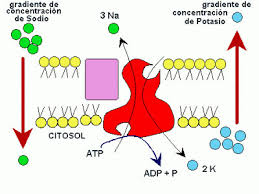
\includegraphics[width=7.5cm]{figures/bomba_sodio.jpeg}
    \caption{Bomba sodio-potasio}
    \label{fig:bomba_sodio_potasio}
\end{figure}
\section{Potencial de acción}
\begin{figure*}[htbp!]
        \centering
        \begin{subfigure}[b]{0.4\textwidth}
            \centering
            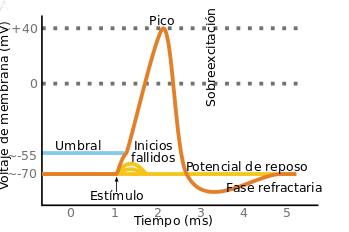
\includegraphics[width=\textwidth]{figures/potencial_accion_esquematico.png}
            \caption{Vista esquemática de un potencial de acción ideal, mostrando las distintas fases}
            \label{fig:potencial_accion_ideal}
        \end{subfigure}
        \hspace{1.25cm}
        \begin{subfigure}[b]{0.4\textwidth}  
            \centering 
            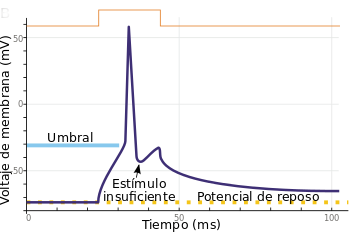
\includegraphics[width=\textwidth]{figures/potencial_accion_real.png}
            \caption{Registro real de un potencial de acción}
            \label{fig:potencial_accion_real}
        \end{subfigure}
        \quad
        \caption{Potencial de acción}
        \label{fig:potencial_accion}
\end{figure*}
Cuando se aplica a una neurona un estímulo de intensidad suficiente para que el potencial de membrana alcance un límite denominado \textbf{umbral}, se genera una señal que recibe el nombre de \textbf{potencial de acción} (ver sitio web \cite{khanacademywebsite}).
Un potencial de acción es un cambio muy rápido en la polaridad de la membrana de negativo a positivo y de vuelta a negativo, en un ciclo que dura unos milisegundos. Cada ciclo comprende una \textit{fase ascendente}, una\textit{ fase descendente} y una \textit{fase hiperpolarizada}.\\
El potencial de acción no se mantiene en un punto de la membrana plasmática, sino que viaja a lo largo de la membrana. Puede desplazarse a lo largo de un axón a mucha distancia.
\newpage
\subsection{Fases del potencial de acción}\label{subsec:fases_potencial_accion}
\begin{enumerate}
\item \textbf{Fase ascendente}: El estímulo que se aplica a una neurona es una despolarización lo suficientemente grande que aumente el voltaje de la membrana y cruce el valor del umbral (generalmente de -55 mV). Cuando el estímulo llega al umbral, provoca que  se abran los canales de $Na^+$ dependientes del voltaje en la membrana, lo cual permite que ingresen varios iones de sodio precipitadamente a la célula. Estos iones de sodio hace que aumente muy rápido el potencial de membrana hasta +40 mV. En el pico del potencial, el potencial de membrana se encuentra cerca del potencial de equilibrio del sodio.
\item \textbf{Fase descendente}: Cuando el potencial llega al pico, el mismo voltaje del estímulo que provocó la apertura de los canales de sodio al alcanzar el umbral, ahora genera el cierre gradual\footnote{\footnotesize El tiempo que transcurre hasta dejar inactivo a los canales de sodio luego del pico, es muy breve. Prácticamente quedan inactivos en el pico.} de los mismos hasta dejarlos inactivos\footnote{\footnotesize Estado inactivo: Deja de circular iones desde o hacia el interior de la célula}. Al mismo tiempo, el voltaje del estímulo abre los canales de potasio, permitiendo que el potasio salga precipitadamente de la célula. El incremento de la permeabilidad del potasio lleva al potencial de membrana cerca del potencial de equilibrio del potasio. El efecto combinado de los cambios en la permeabilidad del sodio y del potasio hacen que el potencial de membrana caiga rápidamente, repolarizando la membrana y generando una \textit{fase descendente} del potencial de acción.
\item \textbf{Fase hiperpolarizada}: El voltaje despolarizado abre canales de potasio adicionales y algunos de estos no se cierran cuando el potencial de membrana vuelve a su potencial de reposo, además se abrieron canales de potasio adicionales en respuesta a la entrada de iones de sodio durante el potencial de acción. La concentración de $k^+$ en el interior de la célula es inusualmente baja, haciendo que el potencial de membrana se acerque mucho más al potencial de equilibrio del potasio. El potencial de membrana va por debajo del potencial de reposo lo cual produce una \textit{hiperpolarización} que persiste hasta que la permeabilidad del potasio regresa a su estado norma. Los canales de potasio se cierran gradualmente, haciendo que se restaure el potencial de membrana hacia el valor del potencial de reposo. Los canales de sodio vuelven a su estado normal \footnote{\footnotesize Estado normal de  los canales de sodio: Permanecen cerrados pero pueden responder al voltaje}.
\end{enumerate}
\subsection{Período refractario}\label{subsec:periodo_refractario}
El tiempo durante el cual es imposible o difícil generar un segundo potencial de acción luego de haber generado uno anteriormente, es el período refractario. Este período se puede superponer con otras fases del potencial de acción.\\
Cada potencial de acción es seguido por un período refractario que puede ser dividido en \textit{período refractario absoluto} y \textit{período refractario relativo}. Estos dos períodos refractarios son debido al cambio de estado de los canales de sodio y potasio.
\begin{itemize}
    \item \textbf{Período refractario absoluto}: Durante este período es imposible generar un potencial de acción. Cuando los canales de sodio quedan inactivos luego del potencial de acción, no se pueden abrir, sin importar cual sea el potencial de membrana porque entran en un estado \textit{inactivo}.
    \item \textbf{Período refractario relativo}: Este período comprende el breve tiempo luego del período refractario absoluto, cuando algunos canales de sodio ya se recuperaron de su inactivación y pueden desencadenar un segundo potencial de acción, de menor amplitud porque hay menos canales de sodio activos y además requiere un estímulo mayor para poder llegar al umbral.
\end{itemize}
\section{Sinapsis química}\label{sec:sinapsis_quimica}
Un sólo axón puede tener múltiples ramificaciones, lo que le permite hacer sinápsis con una o varias células postsinápticas. Del mismo modo, una neurona puede recibir miles de entradas sinápticas de muchas neuronas presinápticas o emisoras diferentes.\\
Dentro de la terminal axónica emisora hay muchas \textit{vescículas sinápticas}. Son esferas membranosas llenas de moléculas de \textit{neurotrasnmisor}. El pequeño espacio entre la terminal axónica de la neurona presináptica y de la membrana de la célula postsináptica se llama \textbf{espacio sináptico}.
\begin{figure*}[h!]
        \centering
        \begin{subfigure}[b]{0.475\textwidth}
            \centering
            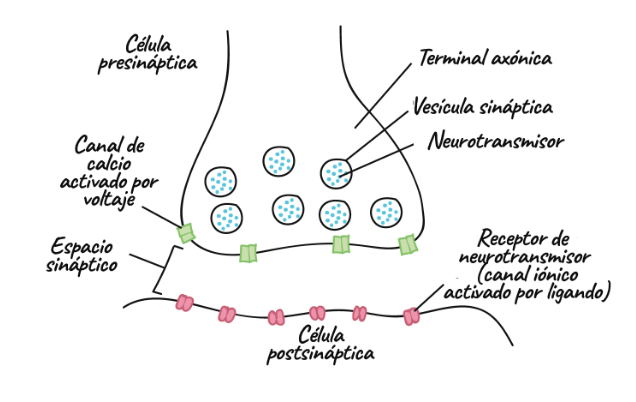
\includegraphics[width=\textwidth]{figures/conexion_neuronas.png}
            \caption{Anatomía de la conexión entre células}
            \label{fig:anatomia_conexion}
        \end{subfigure}
        \hfill
        \begin{subfigure}[b]{0.475\textwidth}  
            \centering 
            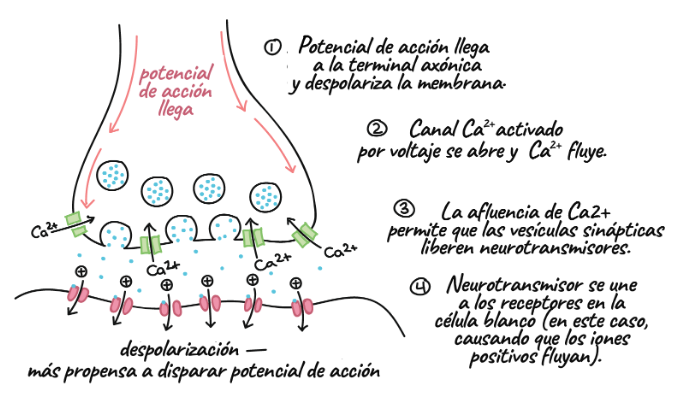
\includegraphics[width=\textwidth]{figures/neurotransmisores.png}
            \caption{Neurotransmisores viajando desde una neurona a otra a través del espacio sináptico}
            \label{fig:neurotransmisores}
        \end{subfigure}
        \quad
        \caption{Conexión entre neuronas}
        \label{fig:conexion_neuronas}
\end{figure*}
Existen muchas \textbf{vescículas sinápticas} dentro de la terminal axónica de una célula emisora (ver figura~\ref{fig:anatomia_conexion}). Son esferas membranosas llenas de moléculas de neurotransmisores. El pequeño espacio entre la terminal axónica de la neurona presináptica y la membrana de la célula postsináptica se llama \textbf{espacio sináptico}.\\
La figura~\ref{fig:neurotransmisores} muestra que cuando llega un potencial de acción o impulso nervioso a la terminal axónica, acciona canales de calcio activados por voltaje en la membrana celular. \newpage
El $Ca^{2+}$ que está muchos más concentrado afuera de la neurona que adentro, entra a la célula. El $Ca^{2+}$ permite que las vescículas sinápticas se fundan con la membrana de la terminal axónica haciendo que se liberen los neurotransmisores en el espacio sináptico. Las moléculas del neurotrasnmisor se difunden por el espacio sináptico y se unen a las proteínas receptoras en la célula postsináptica.\\
Cuando un neurotransmisor se une a su receptor en la célula receptora, causa la apertura o cierre de canales iónicos. Esto puede producir un cambio localizado en el potencial de membrana de la célula receptora.
\begin{itemize}
    \item En algunos casos provoca que la célula sea más propensa a disparar su propio potencial de acción. En este caso el cambio en el potencial de membrana se llama \textbf{potencial excitatorio postsináptico} o \textbf{PEPS}
    \item En otros casos provoca que la célula sea menos propensa a disparar su propio potencial de acción y se llama \textbf{potencial inhibitorio postsináptico} o \textbf{PIPS}
\end{itemize}
Un PEPS es despolarizante: hace que el interior de la célula sea más positivo y acerca el potencial de membrana a su umbral de disparo de un potencial de acción. A veces no es suficiente un PEPS aislado para llevar a la neurona al umbral, pero puede sumarse junto con otros PEPS para desencadenar un potencial de acción.
Los PIPS tienen el efecto contrario. Tienden a mantener el potencial de membrana de la neurona postsináptica por debajo del umbral del potencial de acción. Los PIPS pueden contrarrestar o cancelar el efecto excitatorio de los PEPS.\\
Una neurona postsináptica suma o integra todas las señales inhibitorias y excitatorias que recibe y "decide" si quiere disparar o no un potencial de acción.
\begin{itemize}
    \item La integración de potenciales postsinápticos que ocurren en diferentes lugares pero casi al mismo tiempo se lo conoce como \textbf{suma espacial}. Ejemplo:\\
    suponiendo que en dos dendritas diferentes de la misma neurona postsináptica (marcadas en verde en la figura~\ref{fig:suma_espacial_peps}) se producen sinapsis excitatorias. Ninguna de las dos sinapsis pueden producir un PEPS lo suficientemente grande como para llevar el potencial de membrana al umbral y disparar el potencial de acción. Pero si ambos PEPS se producen al mismo tiempo, podrían sumarse para llevar el potencial de membrana al umbral.
\begin{figure}[htbp!]
    \centering
    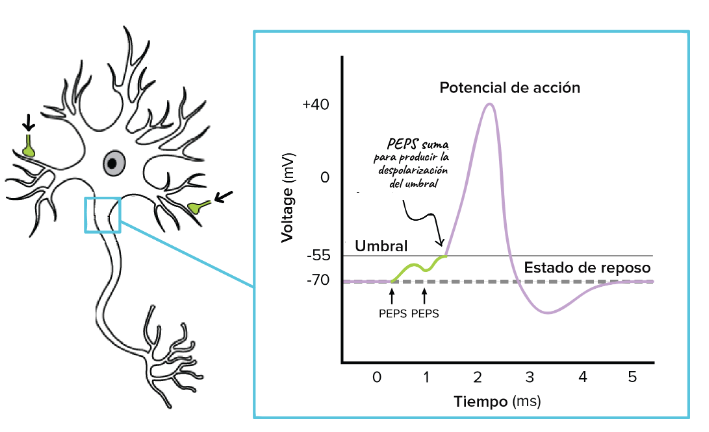
\includegraphics[width=12.0cm]{figures/PIPS_PEPS.png}
    \caption{Suma espacial de PEPS}
    \label{fig:suma_espacial_peps}
\end{figure}
Por otro lado, si ocurrió un PIPS junto con los dos PEPS, podría impedir que el potencial de membrana alcance el umbral y evita que la neurona dispare un potencial de acción. 
    \item La integración de potenciales postsinápticos que ocurren en el mismo lugar pero en momentos ligeramente diferentes se llama \textbf{suma temporal}. Ejemplo:\\
    Si una neurona presináptica se dispara rápidamente dos veces seguidas y causa dos PEPS, el segundo PEPS puede llegar antes que el primero se disipe\footnote{\footnotesize Los potenciales postsinápticos no son instantáneos; por el contrario, duran un ratito antes de disiparse}, lo que lleva el potencial de membrana hacia el umbral.
\end{itemize}
\section{Sinapsis eléctrica}
En las \textbf{sinapsis eléctricas} existe una conexión física directa entre la neurona presináptica y la neurona postsináptica. Esta conexión toma la forma de un canal llamado \textbf{unión de hendidura}, que permite que la corriente -los iones- fluyan directamente de una célula a otra (ver figura~\ref{fig:sinapsis_electrica}).Las sinapsis eléctricas transmiten señales con mayor velocidad que las sinapsis químicas.
\begin{figure}[htbp!]
    \centering
    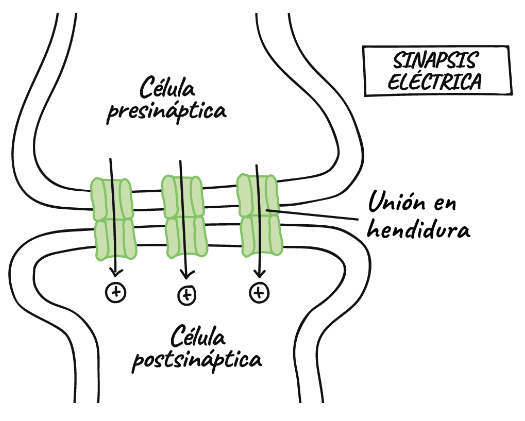
\includegraphics[width=6.5cm]{figures/Sinapsis_electrica.png}
    \caption{Sinapsis eléctrica}
    \label{fig:sinapsis_electrica}
\end{figure}
